%% PNAStwoS.tex
%% Sample file to use for PNAS articles prepared in LaTeX
%% For two column PNAS articles
%% Version: Apr 15, 2008


%% BASIC CLASS FILE
\documentclass{pnastwo}

%% ADDITIONAL OPTIONAL STYLE FILES
%\usepackage[dvips]{graphicx}
%\usepackage{pnastwoF}
\usepackage{amssymb,amsfonts,amsmath}

\newcommand{\red}[1]{{\bf \color{red} #1}}
\newcommand{\blue}[1]{{\bf \color{blue} #1}}
\newcommand{\green}[1]{{\bf \color{green} #1}}

\newcommand{\fixme}[1]{\red{[#1]}}
\newcommand{\davidsays}[1]{{\color{red} [\green{David:} \emph{#1}]}}
\newcommand{\renesays}[1]{{\color{red} [\blue{Rene:} \emph{#1}]}}
\newcommand{\jeffsays}[1]{{\color{red} [\blue{Jeff:} \emph{#1}]}}

\newcommand\micron{\ensuremath{\mu\text{m}}}


%% OPTIONAL MACRO DEFINITIONS
%\def\s{\sigma}


%%%%%%%%%%%%
%% For PNAS Only:
\url{www.pnas.org/cgi/doi/10.1073/pnas.0709640104}
\copyrightyear{2008}
\issuedate{Issue Date}
\volume{Volume}
\issuenumber{Issue Number}
%\setcounter{page}{2687} %Set page number here if desired
%%%%%%%%%%%%

\begin{document}

\title{Robustness of MinD oscillation in \emph{Escherichia coli} with
  diverse cell shapes}

\author{Jeff B. Schulte\affil{1}{Department of Physics, Oregon State University},
Rene W. Zeto\affil{1}{}
\and
David Roundy\affil{1}{}}

\contributor{Submitted to Proceedings of the National Academy of Sciences
of the United States of America}

\significancetext{When an E. Coli cell divides it must split into two
  relatively equal volumes in order to survive.  One mechanism that
  aids in this process is a system of proteins that oscillate between
  cell ends and help the original cell divide along it’s center.  A
  recent experiment found that by drastically deforming these cells
  this oscillation can be disrupted.  We examine these oscillations in
  similarly deformed cells computationally, using two widely used
  simulation models, and find good agreement using one of them.  The
  other model fails in a manner far more dramatic than has been
  previously observed.  Furthermore, we find that the effect observed
  experimentally in asymmetric and flattened cells is primarily a
  result of the flattening, not the asymmetry.  }

\maketitle

\begin{article}
\begin{abstract}
  The dynamics of the Min-protein system help \emph{Escherichia coli}
  regulate the process of cell division by identifying the center of
  the cell.  While this system usually exhibits robust polar
  oscillations in a variety of cell shapes, new experiments have shown
  that when the cells are mechanically deformed into wide, flattened
  out, irregular shapes, the spatial regularity of these oscillations
  breaks down. Here we study widely used stochastic and deterministic
  models of Min-system simulation within these new cell shapes.  We
  find that the deterministic model is decidedly inadequate to
  reproduce the experimentally observed behavoir, while the stochastic
  model, based on the same differential equations, is able to do so
  accurately.  We also find that it is the flattening rather than the
  irregularity and asymmetry of the cell shape that causes the
  irregular oscillation behavoir.
\end{abstract}

\keywords{MinD | \emph{Escherichia coli} | stochastic | deterministic }

%% \abbreviations{SAM, self-assembled monolayer; OTS,
%% octadecyltrichlorosilane}

\dropcap{I}t is vital that during the process of bacterial cell
division a cell avoid minicelling, or splitting into daughter cells
with lopsided volumes.  Instrumental to this process in
\emph{Escherichia coli} is a long FtsZ polymer chain that develops on
the cell wall in the center region of the cell, helping dictate the
plane of division~\cite{adams2009bacterial,
  lutkenhaus2007assembly}. Previous experimental studies have shown
that the MinC protein, known to inhibit the FtZ
polymer~\cite{shen2010examination}, exhibits regular pole to pole
oscillatory behavior between both ends of the wild-type pill-shaped
cell.  It thus has a higher time averaged concentration in the cell
poles than in the center region, which aides in preventing the FtZ
from developing in the wrong region.  The MinC is recruited to these
poles by MinD, which itself interacts with another protein, MinE, in a
system which exhibits pole-to-pole oscillatory
behavoir~\cite{shapiro2009and, yu1999ftsz,
  meacci2005min,huang2003dynamic,kerr2006division,mannik2009bacterial}.
%% \cite{hu1999topological, fu2001mine, shapiro2009and,
%%   yu1999ftsz, raskin1999rapid, meacci2005min, raskin1999minde}.

Previous experimental studies have shown that the MinD protein system
is capable of exhibiting oscillations in round
shapes~\cite{fange2006noise} as well as in connected three pronged
tube shapes~\cite{varma2008min}, in which the oscillations seem to
seek out the extreme poles in the cell.  One conclusion of these
studies has been that the MinD system robustly forms bipolar
oscillations regardless of variations in cellular shape.

However, Mannik \emph{et al.} have recently shown that there are
limitations to this robust capability to
oscillate~\cite{mannik2010bacteria, mannik2009bacterial}. They have
experimentally forced \emph{E. coli} cells into microfabricated
silicon channels of $0.25\micron$ thickness. Upon entering the
channels, the cells undergo a mechanical deformation in which they
both widen and lengthen within the plane of the channel.  This
deformation results in very wide (they can reach widths of over
$5\micron$) flattened cells that when viewed from the top down have
irregular and asymmetric shapes.  While these cells are still able to
divide into surprisingly equal volumes, the MinD oscillations in these
cells are irregular, both temporally and spatially. Seen with
flourescent microscopy, the MinD maximize in multiple locations within
the cell, in a seemingly random sequence. These experiments allow for
an opportunity to test MinD simulation models against more extreme
cases than have been seen thus far.

A number of models of the MinD protein system have been developed,
which accurately describe the dynamics using simulations of
reaction-diffusion equations.
%
Early models involved free proteins that affect each others' rates of
diffusion and membrane attachment, but do not combine into compound
states~\cite{meinhardt2001pattern}.  In 2003 Huang improved upon this
work with a simple and very successful simulation model based on
MinD-MinE combination, ATPase hydrolysis, and MinD membrane attachment
that exhibits accurate MinD oscillations in cylindrical
cells~\cite{huang2003dynamic}. In this model cytoplasmic MinD is
recruited to the membrane by MinD that is already clustered there
(following observed non-linear attachement of MinD on the cell
membrane~\cite{hu2002dynamic,shih2002division}), and is stationary
once attached.  A number of studies have used an approach similar in
that they do not rely on the ability of MinD to move along the walls
and cluster~\cite{kruse2007experimentalist, meinhardt2001pattern,
  drew2005polymerization, fange2006noise, kerr2006division}, while
studies have been made as well of models which rely on MinD mobility
and attraction on the cell membrane~\cite{kruse2002dynamic,
  howard2005cellular}.

There are only on the order of 1000 MinD proteins in a given cell,
which means that stochastic fluctuation can be expected to play a
large role.  To treat this, there have been a number of variations of
the Huang 2003 model that stochastically simulate the same
reaction-diffusion equations~\cite{fange2006noise, kerr2006division}.
These studies largely confirm the results of Huang's deterministic
model when applied to the wild-type, pill-shaped phenotype.  However,
the stochastic models are slightly more successful in predicting
experimentally observed oscillations in round cell
phenotypes~\cite{fange2006noise, huang2004min}, and they enable
prediction of fluctuations in the predicted
behavior~\cite{kruse2007experimentalist}.  Both deterministic and
stochastic models are widely used throughout systems
biology~\cite{lawson2013spatial, robb2014stochastic,
  oguz2014stochastic, fu2013deterministic, rudiger2014stochastic}, and
have unique advantages and limitations.  The deterministic approach
has an advantage in providing a simple prediction of average behavior,
while the stochastic approach enables prediction of fluctuations from
that mean, and reduces sensitivity to initial conditions.

%% biology~\cite{lawson2013spatial, robb2014stochastic,
%%   oguz2014stochastic, fu2013deterministic, rudiger2014stochastic}, and
In this paper we use Huang's 2003 model~\cite{huang2003dynamic} in
both deterministic and stochastic variants to study flattened cells
similar to those observed by Mannik~\cite{mannik2009bacterial}.

\begin{figure}
  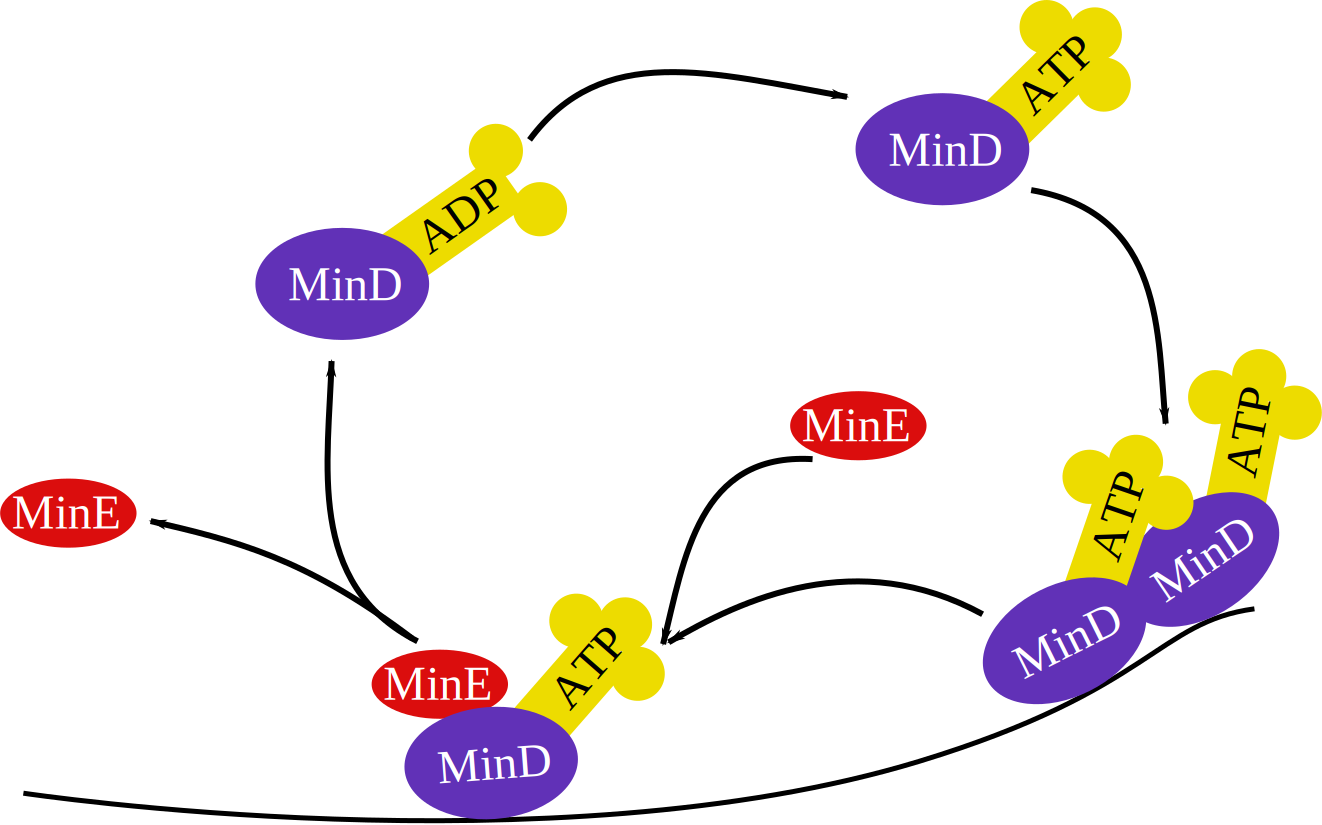
\includegraphics[width=8.7cm]{reactions}
  \caption{Reactions included in the model of Huang \emph{et
      al.}~\cite{huang2003dynamic}.}\label{fig:reactions}
\end{figure}


\section{Model, Methods, and Cell Shapes}\label{sec:model-method-shapes}
We implement the reaction-diffusion model of Huang \emph{et
  al.}~\cite{huang2003dynamic}.  Figure~\ref{fig:reactions} shows the
reaction process.  The cytoplasmic MinD:ADP complex undergoes
nucleotide exchange and is changed into the MinD:ATP complex.  This
will naturally diffuse and attach to the cell membrane.  A cytoplasmic
MinE will attach to the wall bound MinD:ATP complex and after a time
will activate ATP hydrolosis.  This breaks up the complex, releasing
MinE, phosphate, and MinD:ADP back into the cytoplasm.  The MinD:ADP
will undergo nucleotide exchange and begin again the cyclic process.
The model is defined by a set of five reaction-diffusion equations:

\begin{multline}
  \frac{\partial \rho_{D:ADP}}{\partial t} = \mathcal{D}_D\nabla^2\rho_{D:ADP}-k_D^{ADP\rightarrow ATP}\rho_{D:ADP}\\
  +\delta(d_w)k_{de}\sigma_{DE},\hspace{3.4cm}
\end{multline}
\begin{multline}
  \frac{\partial \rho_{D:ATP}}{\partial t} = \mathcal{D}_D\nabla^2\rho_{D:ATP}+k_D^{ADP\rightarrow ATP}\rho_{D:ADP}\\
  -\delta(d_w)[k_D+k_{dD}(\sigma_D+\sigma_{DE})]\rho_{D:ATP}
\end{multline}
\begin{multline}
  \frac{\partial \rho_E}{\partial t} = \mathcal{D}_E\nabla^2\rho_E+\delta(d_w)k_{de}\sigma_{DE}
  -\delta(d_w)k_E \sigma_D \rho_E
\end{multline}
\begin{multline}
  \frac{\partial \sigma_D}{\partial t} = -k_E\sigma_D\rho_E
  +[k_D+k_{dD}(\sigma_D+\sigma_{DE})]\rho_{D:ATP}
  \label{eq:d-on-wall}
\end{multline}
\begin{multline}
  \frac{\partial \sigma_{DE}}{\partial t} = -k_{de}\sigma_{DE}+k_E\sigma_D\rho_E\hspace{3cm}
  \label{eq:FifthPDE}
\end{multline}
where $\rho$ is cytoplasmic protein density (proteins$/\micron^{3}$), $\sigma$
is membrane bound density (proteins$/\micron^{2}$), $\mathcal{D}_D$ and
$\mathcal{D}_{E}$ are the diffusions constants for MinD and MinE,
respectively, $k_D^{\textrm{ADP $\rightarrow$ ATP}}$ is the rate of
conversion from MinD:ADP to the MinD:ATP complex, $k_D$ is the rate of
MinD:ATP attachement to the membrane when no protein is already
attached there, $k_{dD}$ is the increase of this rate when MinD:ATP is
present on the membrane, $k_{de}$ is the rate of hydrolisis of the
MinD:MinE:ATP complex, $k_E$ is the rate of cytoplasmic MinE binding
to membrane bound MinD:ATP complex, and $d_w$ is the distance from the
point in space to the closest wall.  The Dirac delta function
$\delta(d_w)$, which we need to describe the location of the membrane,
has units of $\micron^{-1}$ and is zero everywhere except at the wall.
Equations \ref{eq:d-on-wall} and \ref{eq:FifthPDE} are only relevent
at the membrane because the membrane-bound density values have no
meaning in the cytoplasm.

Our diffusion and reaction rates are shown below.  We are interested
primarily in the effect of cellular size and shape on the protein
oscillations, so we follow Huang\cite{huang2003dynamic} and do not
deviate from the wild-type values used in the cited work.

\begin{gather*}
  \mathcal{D}_D = \mathcal{D}_{E} = 2.5\micron^2/\text{sec}\\
  k_D^{\textrm{ADP $\rightarrow$ ATP}} = 1/\textrm{sec,  }
  k_D = 0.025 \micron /\textrm{sec}\\
  k_{dD} = 0.0015 \micron^3/ \textrm{sec,  }
  k_{de} = 0.7/\textrm{sec}\\
  k_E = 0.093 \micron^3 /\textrm{sec}.
\end{gather*}

Huang's simulations use total MinD and MinE concentrations of
$1,000/\micron$ and $350/\micron$, respectively, in a cylindrical cell
of radius $0.5\micron$, and in our (non-cylindrical) cells we use the
same number of proteins per unit volume.  These concentration values
are $1273\micron^{-3}$ and $446\micron^{-3}$, respectively. We perform
simulations with a 3D grid in cartesian coordinates that has a grid
spacing of .05\micron.

We have performed both a numerical, deterministic model simulation
that is spatially and temporally discrete, and a stochastic simulation
that is spatially discrete but continuous in time.  Our stochastic
model follows the work of Kraus~\cite{kraus1996crosstalk} which in
turn follows a method introduced by
Gillespie~\cite{gillespie1977exact}.

We mean to investigate the geometric limits of the Min system
oscillations as observed by Mannik \emph{et
  al.}~\cite{mannik2012robustness}, so we have modeled the Min system
in several cell shapes and sizes.  Here we present a selection of
these, beginning with naturally occuring pill-shaped cells, followed
by a number of flattened out shapes which reflect the experiments of
Mannik \emph{et al.}, in which bacteria are confined within a thin
slit of height $0.25\micron$ ~\cite{mannik2012robustness}.  Viewed
from the top down the cells have the shapes described below and viewed
from the side they have at their edges a semicircular protrusion (one
may imagine the shape of a pancake).
%
In this paper we focus on four specific flattened cell shapes.  Two of
these shapes replicate those published by Mannik, and the other two
are `stadium' shapes that respectively have the same aspect ratio,
thickness, and volume as the two Mannik shapes.  Viewed from the top
down, these stadium shapes appear as rectangles with semi-circular end
caps on the long axis ends.

\begin{figure*}
  %\includegraphics[width=\textwidth]{../data/shape-p/3_00-0_50-0_00-0_00-15_00-exact/plots/image-plot}
  \begin{center}
    \includegraphics[height=6.4cm]{../data/shape-p/3_00-0_50-0_00-0_00-15_00-exact/plots/single-image-plot}\\
    \vspace{-1.5em}
    \includegraphics[height=6.4cm]{../data/shape-p/3_00-0_50-0_00-0_00-15_00-full_array/plots/single-image-plot}
    \vspace{-1.5em}
  \end{center}
  \caption{Images of the concentration of each protein species in a
    natural pill-shaped bacterium at one-second time intervals. The
    upper plots shows results from the deterministic model and the
    lower shows results from the stochastic model.  The order of
    frames is such that individual MinD proteins begin at the bottom
    of the plot (in the MinD:ATP state in the cytoplasm), and progress
    upward until they reach the MinE:MinD:ATP membrane-bound complex.
    At that point, they will spontaneously dissociate into cytoplasmic
    MinE (the top row) and the starting state of cytoplasmic
    MinD:ADP.}.
  \label{image-p}
\end{figure*}

Huang \emph{et al.}~\cite{huang2003dynamic} has performed a linear
stability analysis on a cylindrical model which shows an upper limit
on a steady state solution of a $2\micron$ half wavelength.  Cells
with dimensions longer than this show spontaneous oscillatory behavoir
in this direction, while cells that are shorter relax into a
motionless steady state.  We have similarly performed a linear
stability analysis on an infinite slab with a thickness equal to that
of our flattened cells ($0.25\micron$) and have found that an
equivalent stability limit for half wavelength is $2.13\micron$. As
expected, when decreasing the lengths and widths of our simulated
flattened cells so that the longest distance across the cell is less
than this length, the cells stop exhibiting any oscillatory behavior.
The deterministic model relaxes into a motionless state and the
stochastic model exhibits random fluctuations without spatial
oscillations.

\section{Naturally Occuring Pill Shaped Cells}

\begin{figure}
  \begin{center}
    \includegraphics[height=6.4cm]{../data/shape-p/3_00-0_50-0_00-0_00-15_00-full_array/plots/correlation.pdf}
  \end{center}
  \caption{Temporal correlation function of the total MinD found in
    two opposite polar regions of the pill-shaped cell, shown against
    the correlation time.  Data for both the the determinisitic and
    stochastic models are shown.  The stochastic model shows an
    oscillation period of 39.5 seconds and coherence time of 307 seconds.
    The correlation functions are scaled to have the same initial
    value.}
  \label{corr-pill}
\end{figure}

We begin with the naturally occuring pill cell shape.  We piece this
shape together as a cylinder with hemispherical endcaps.  This shape
follows the early simulations of Huang \emph{et al.} but differs in
that we have added the end caps for a more natural shape, expecting
similar results.

Figure~\ref{image-p} shows a series of color plots of the density of
proteins at each stage of the reaction cycle. Deterministic simulation
data is shown above and stochastic simulation data is shown below.
The cells shown are $4\micron$ in length, measured from end to end.
We have `smeared out' the stochastic concentrations in a manner meant
to reproduce the images shown by diffraction limited flourescence
microscopy.  We do so using the two dimensional gaussian approximation
developed by Zhang \emph{et al.}~\cite{zhang2007gaussian}.  In this
approximation we use a numerical aperture value of 1.3, which is the
same as used by Mannik experimentally, and a wavelength of $650nm$.
Each frame is 2.5 seconds ahead of the last, and each image shows the
concentration of a given state of protein (of the five described in
the reaction model) summed over the coordinate normal to the page.

Figure~\ref{image-p} begins about 300 seconds into the simulation and
shows one period of oscillation.  At $t=0$ there is a high
concentration of MinD:ATP that has accumulated on the membrane at the
bottom of the cell. An important aspect of Huang's model is that the
MinD is attracted to and sticks to the membrane nonlinearly: as it
accumulates there it begins to `recruit' other MinD that is diffusing
in the cytoplasm nearby, causing peaks in concentration to build up on
the walls.  Meanwhile, the MinE creeps downward as it reacts with the
membrane-bound MinD, forming the MinD:MinE:ATP complex, then breaks it
apart and diffuses downward a bit more before it again reacts with
membrane-bound MinD.  This process can be seen in the form of the
well-known ``MinE rings'' (actually, MinE bound to MinD on the
membrane).  These rings are visible in the deterministic model plots
as a green band on the walls from 0 seconds to 4 seconds (and later
from 15 to 23 seconds).  The appearence of these rings in the
deterministic model along side their less obvious appearence in the
stochastic model highlights an advantage of the deterministic model:
the idealization of deterministic data allows one to see patterns in
the averaged behavior that might otherwise be missed.  In the
stochastic model the MinE still exhibits higher concentrations in the
same regions throughout the process, but what would ideally be a
``ring'' pattern is instead an asymmetric collection of maxima, which
would become a ring after phase-locked averaging.

During the formation of these rings, cytoplasmic MinE is diffusing in
the upper portion of the cell and will naturally progress downward,
where there is membrane-bound MinD to react with, leading to a
depletion of MinE in the upper portion of the cell.  As the MinE ring
converges upon the lower end of the cell, MinD that has been released
is able to diffuse upward, past the ring, while still in its MinD:ADP
state and unable to bind to the membrane.  After it undergoes
nucleotide exchange, resulting in MinD:ATP, it is ready to accumulate
on the walls in at the top of the cell, where the MinE has been
depleted.  This can be seen in seconds 10 through 20 in both models,
followed by the subsequent MinE ring formation and movement upward
(beginning the same process in the opposite direction) that can be
seen in seconds 15 through 23.

It is clear from Fig.~\ref{image-p} that the stochastic simulation
results in a protein distribution that is less spatially regular than
the deterministic model predicts.  In fact, when viewed as a movie
(see supplementary material), the stochastic model exhibits a ``starry
night'' effect, as recruitment leads to clusters of MinD forming on
the wall and then subsequently dissipating.  This naturally leads to
irregularity in the temporal periodicity of the system, which we
quantify by examining the temporal correlation function of the total
MinD found in two opposite polar regions.
%
This correlation function, which is displayed in Fig.~\ref{corr-pill},
is given by
\begin{equation}
  C(\tau) \propto \int
  (N_{\textit{top}}(t) - \bar N_{\textit{top}})
  (N_{\textit{bottom}}(t+\tau) - \bar N_{\textit{bottom}})dt
\end{equation}
where $N_{\textit{top}}(t)$ and $N_{\textit{bottom}}(t)$ are the total
MinD proteins in the top and bottom thirds of a cell.  These plots
help us in studying the periods and the regularity and stability of
oscillations.  These curves are well fit with a simple decoherence
model, given by the equation
\begin{equation}
  C(\tau) = -\cos\left(\frac{2\pi\tau}{T}\right) e^{-\frac{\tau}{\tau_c}}
\end{equation}
where $T$ is the period and $\tau_c$ is the coherence time.  In the
case of the stochastic model the pill exhibits coherence times of
about 8 periods and in the case of the determinisitic model oscillate
indefinitely with complete coherence, indicating that its behavior is
perfectly periodic.

\begin{figure*}
  \centering
  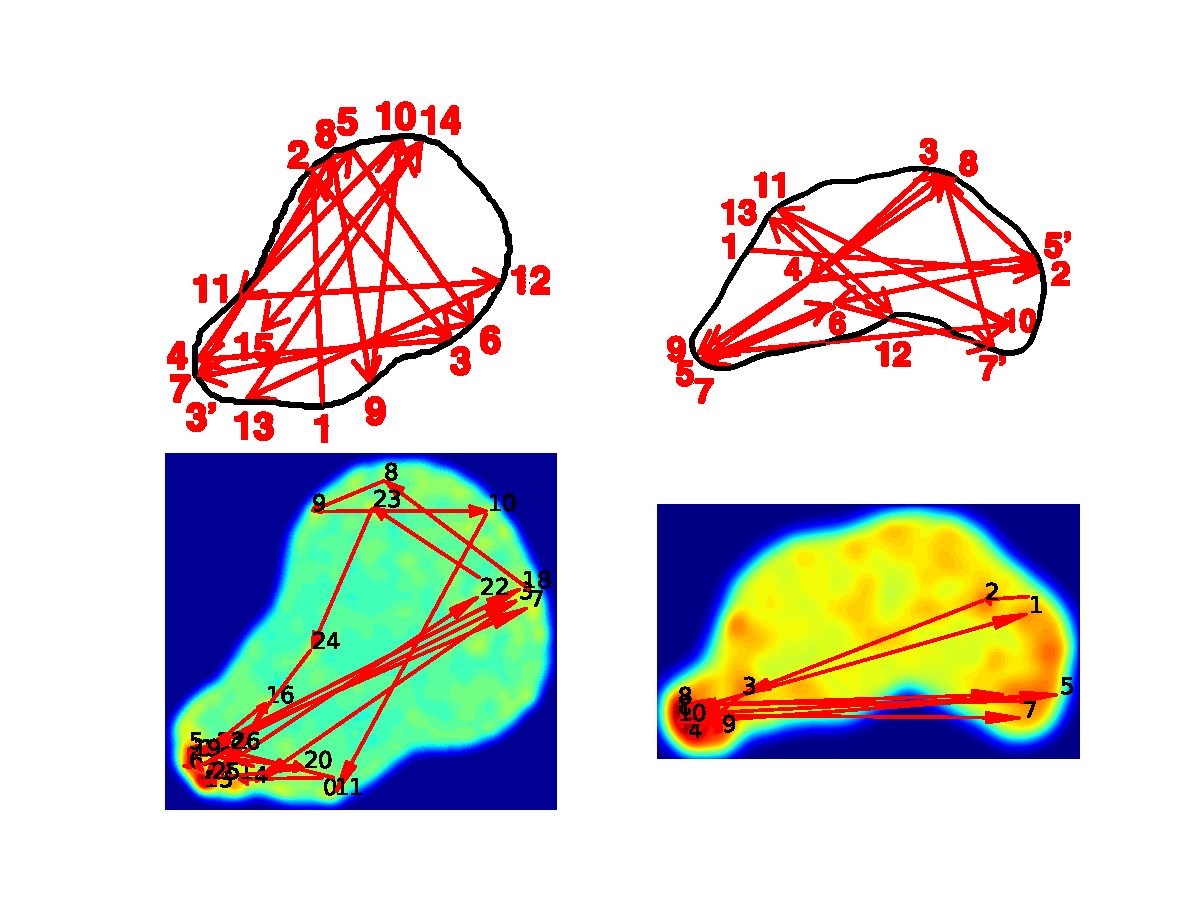
\includegraphics[width=16cm]{../paper/plot-ave}
  \caption{We display here arrows depicting successive maxima in space
    and and time overlayed on a color plot of the total MinD density
    averaged over the same time period.  The simulation time covered
    for the flattened cells is 350 seconds, which is the same
    period of time depicted in the experimental data plots of Mannik
    \emph{et al.}~\cite{mannik2012robustness}.  For the wild-type pill
    shape, we only cover 250 seconds, in order to provide a
    useful comparison due to its shorter oscillation period.  The top
    row shows plots published by Mannik of the MinD maxima behavoir
    and the bottom two rows show our simulations using the stochastic
    and deterministic models, respectively.  We simulated
    approximations to the two shapes observed by Mannik, which we call
    \emph{shape A} and \emph{shape B}.  In addition, we studied two
    flattened stadium shapes which we call \emph{stadium A} and
    \emph{stadium B} corresponding in aspect ratio and thickness to
    the two experimental shapes.  The spatial length scale of all the
    figures shown was identical. Each of the flattened cell shapes
    uses the same color scale for the number of proteins per unit
    area.  Finally, we display the natural pill shape, which was also
    featured in Figs.~\ref{image-p} and~\ref{corr-pill}, with a
    different color scale to reflect the thicker cell containing more
    proteins per cross-sectional area.  }
  \label{randst-plot-ave}
\end{figure*}

\begin{figure}
  \begin{center}
    \includegraphics[height=6.4cm]{../data/shape-randst/0_25-18_50-18_50-95_00-15_00-full_array/plots/correlation.pdf}\\
    \includegraphics[height=6.4cm]{../data/shape-stad/0_25-2_35-1_32-0_00-15_00-full_array/plots/correlation.pdf}
  \end{center}
  \caption{Temporal correlation function of the total MinD found in
    two opposite polar regions of the shape \emph{A} (above) and the
    stadium \emph{A} (below) cell shapes, shown against the
    correlation time.  Data for both the the determinisitic and
    stochastic models are shown, and the correlation functions are
    scaled to have the same initial value.  For shape \emph{A}, the
    stochastic model shows an oscillation period of 53.1 seconds and
    coherence time of 246 seconds, so that it takes roughly 4.6 periods
    for the behavoir to decohere.  For the stadium \emph{A}, the same
    model shows an oscillation period of 51 seconds and coherence time of
    323 seconds, so that it takes roughly 6.3 periods for the behavoir
    to decohere.}
  \label{fig:corr-pancake-A}
\end{figure}

\section{Comparison of Mannik's Experimental and Our Stadium Shapes}
As described in Section~\ref{sec:model-method-shapes}, we will focus
on simulation of four illustrative flattened cell shapes: two shapes
created to replicate those shapes observed experimentally by
Mannik~\cite{mannik2012robustness} (shape~\emph{A} and
shape~\emph{B}), and for comparison two symmetrical stadium shapes
that have the identical aspect ratio, thickness and volume (stadium
\emph{A} and stadium \emph{B}), shown in Figure~\ref{randst-plot-ave}.
These stadium shapes enable us to distinguish between the effect of
flattening the cell and the cell shape's irregularity and asymmetry.
We note that shape \emph{B} is more irregular than shape \emph{A}, and
in particular features a prominant region of concavity on its
left-hand side.  For each of these shapes (in addition to the
wild-type pill shape discussed previously) we have simulated in excess
of 15000 seconds (over 4 hours) of evolution of the MinD system using
the deterministic version of Huang's model~\cite{huang2003dynamic},
and in excess of 100000 seconds (over 27 hours) using the stochastic
model.

From each of these flattened simulations, we have chosen a typical 350
second segment to compare with the puplished results of
Mannik~\cite{mannik2012robustness}, exemplified in arrow plots in
which the arrow heads show the location of sequential MinD maxima
within the cell (in Fig.~\ref{randst-plot-ave}).  In addition to
arrows between successive maxima in space and time, we plot as a
colored background the density of MinD protiens averaged over the same
time period.  We note that we have manually verified that our
(computer-generated) arrow plots also reflect a human interpretation
of a movie of the same data.  Finally, for comparison we present the
same plot for a wild-type cell, with a time period of 250 seconds to
account for its short period of oscillation.

In every case, including the wild-type pill shape, we see irregularity
in the location of the maxima when using the stochastic model.  The
deterministic model shows uniformly bipolar oscillation, with the
exception of shape \emph{B}, which develops weak intermediate maxima
on the right-hand edge of the cell.  From these results, we conclude
that the deterministic model is inadequate to explain experimental
observations of the locations of density maxima of the MinD protein.

%% We found that the deterministic simulations of the MinD system results
%% in robust and regular oscillatory behavoir of polar selection and
%% oscillation in not only symmetrical shapes, such as the wildtype pill
%% shape, but also in very assymetrical, flatttened cells, such as those
%% observed by Mannik.  We also examined larger and smaller versions of
%% these shapes, and found this behavior to be very robust, from the
%% minimum size to sustain oscillation (around \fixme{???} $\mu$m) up to
%% around twice the cell size reported by Mannik.  At larger sizes than
%% this, less regular oscillations occur using the deterministic method,
%% but we note that the cells reported by Mannik are already considerably
%% larger in volume than typical wild type
%% cells~\cite{kubitschek1990cell,kubitschek1968linear,mannik2012robustness}.

The predictions of the stochastic model are roughly similar to the
experimental results in terms of irregularity of the locations of
maxima, although there are locations on the edges of the cells where
experiment shows maxima occuring that we never see in our simulations,
suggesting that the model does not precisely reflect the experiment.
We also note that the stadium shapes in Fig.~\ref{randst-plot-ave}
appear to have maxima location irregularity that is qualitatively
similar to our Mannik shapes and to experiment.

However Fig.~\ref{randst-plot-ave} leaves unclear the importance of
the flattening of the cell versus cell shape irregularity and
asymmetry in developing an understanding of the origin of the
experimentally observed behavior.  Although in the movies the stadiums
appear to display, on average over long time scales, a more regular
bipolar oscillation than the irregular mannik shapes, the limited time
range of the arrow plots (350 seconds) is inadequate when studying
this difference in behavoir.  We therefore return to the correlation
function between the number of proteins in a segment at the top of the
cell and the number of proteins in a segment at the bottom of the
cell.  Fig.~\ref{fig:corr-pancake-A} shows this plot for shape
\emph{A} and stadium \emph{A}.  E. Coli cell doubling times vary
widely depending on environmental conditions, but will often be
between 20 minutes to 100 minutes~\cite{pierucci1972chromosome}, while
flourescent microscopy experiments have shown that the FtsZ ring
builds itself with a half life of roughly 30
seconds~\cite{stricker2002rapid}.  Here we plot correlations of
correlation times up to 500 seconds, a biologically relevent
timescale.

%% \begin{figure}
%%   \includegraphics[width=8.7cm]{../data/shape-randst/0_25-18_60-28_60-94_00-15_00-full_array/plots/correlation.pdf}
%%   \includegraphics[width=8.7cm]{../data/shape-stad/0_25-2_92-1_18-0_00-15_00-full_array/plots/correlation.pdf}
%%   \caption{Correlation for B shapes}
%%   \label{corr-B}
%% \end{figure}

We see that both in the shape \emph{A} and stadium \emph{A}, the
deterministic model is perfectly periodic.  Both the deterministic and
stochastic model correlations have the same number of proteins in
their cells, and have been normalized with the same normalization
factor, so that they can be directly compared against eachother.  The
stochastic simulation of shape \emph{A} has a coherence time of 4.6
periods, while the corresponding simulation of stadium \emph{A} has a
coherence time of 6.3 periods.
%
The correlation function for stadium \emph{B} is similar to that of
stadium~\emph{A}, with similar coherence time (5.5 periods, not
shown), while shape~\emph{B} exhibits a lower coherence time (2.2
periods).  In the deterministic model, shape~\emph{B} is not precisely
periodic on biologically relevant timescales, which is reflected in
Fig.~\ref{randst-plot-ave}, in which the arrows describing the
deterministic model applied to shape \emph{B} show minor maxima
forming on the right-hand side of the cell, in contrast to the regular
polar maxima formed by shape~\emph{A} and the two stadiums.
%
From the stochastic correlation data, we conclude that irregularity of
shape has only a moderate affect on the temporal regularity of the
oscillatory behavior, with even the very distorted shape~\emph{B}
exhibiting only a factor of two greater decoherence.

\section{Conclusion}

We find agreement between our stochastic simulations and experiments
showing disrupted bipolar MinD oscillation in asymmetric flattened
E. coli cells~\cite{mannik2012robustness}.  As observed
experimentally, our simulations predict that MinD maxima will form in
a spatially irregular sequence of locations.  This result builds upon
existing results showing that this model is effective in a variety of
wild-type and mutated cell shapes~\cite{fange2006noise, varma2008min,
  kruse2007experimentalist}, and reinforces that the stochastic
variation of Huang's 2003 model~\cite{fange2006noise,
  kerr2006division} has considerable predictive power beyond the
standard wild-type cell.


%
%% We have simulated flattened cell shapes similar to those observed
%% experimentally by Mannik \emph{et al.}, with a stochastic and a
%% deterministic version of Huang's widely used reaction-diffusion model.
%% %
%% We find that the stochastic model predicts experimentally accurate
%% qualitative behavoir in both the wild-type, pill-shaped cells (as
%% found in previous studies~\cite{fange2006noise, varma2008min,
%%   kruse2007experimentalist}), as well as in the new, flattened,
%% irregularly shaped cells.  These flattened cells invariably show
%% spatially irregular formation of maxima as has been observed
%% experimentally.

In contrast to the stochastic model, the original deterministic
version of the model~\cite{huang2003dynamic} predicts behavior that
contradicts experimental observations, namely robust and periodic
bipolar oscillation in irregularly shaped cells, with a minor
intermediate maximum appearing in shape \emph{B}.  Thus we conclude
that this method is inconsistent with experiment, and cannot be relied
upon for predictions of the behavior of the MinD system.  This is the
most clear example of the inadequacy of the deterministic simulation
method in reproducing experimental behavoir of the MinD system to
date.  Until now the results of deterministic and stochastic
simulation have largely coincided, with the stochastic method showing
minor differences in behavoir when compared to deterministic
models~\cite{kerr2006division, fange2006noise, huang2004min,
  kruse2007experimentalist}.

We find that flattened but regular and symmetric cells exhibit MinD
oscillations that are qualitatively similar to the oscillations
observed experimentally (and in our simulation) in irregular and
asymmetric cells.  This demonstrates that asymmetry is not required in
order to induce spatially irregular MinD oscillations.  In addition,
the temporal regularity of oscillations is only moderately affected by
irregularity in the shape of flattened cells.  Thus we conclude
that it is the flattening of the cells rather than their irregular
shape that primarily causes the spatial irregularity of maxima which
is observed by Mannik \emph{et al.}~\cite{mannik2012robustness}.

%% %\section*{Appendix}
%% \begin{acknowledgments}
%% This work was partially supported by
%% Spanish Ministry of Science and Technology Grant BFM2002-02042 (to D.C. and
%% J.L.R.) and by National Science Foundation Grand DMS-0245242 (to C.F.).
%% \end{acknowledgments}

\bibliographystyle{plain}
\bibliography{paper-MinD}
\end{article}

%% \clearpage

%% \begin{figure}
%%   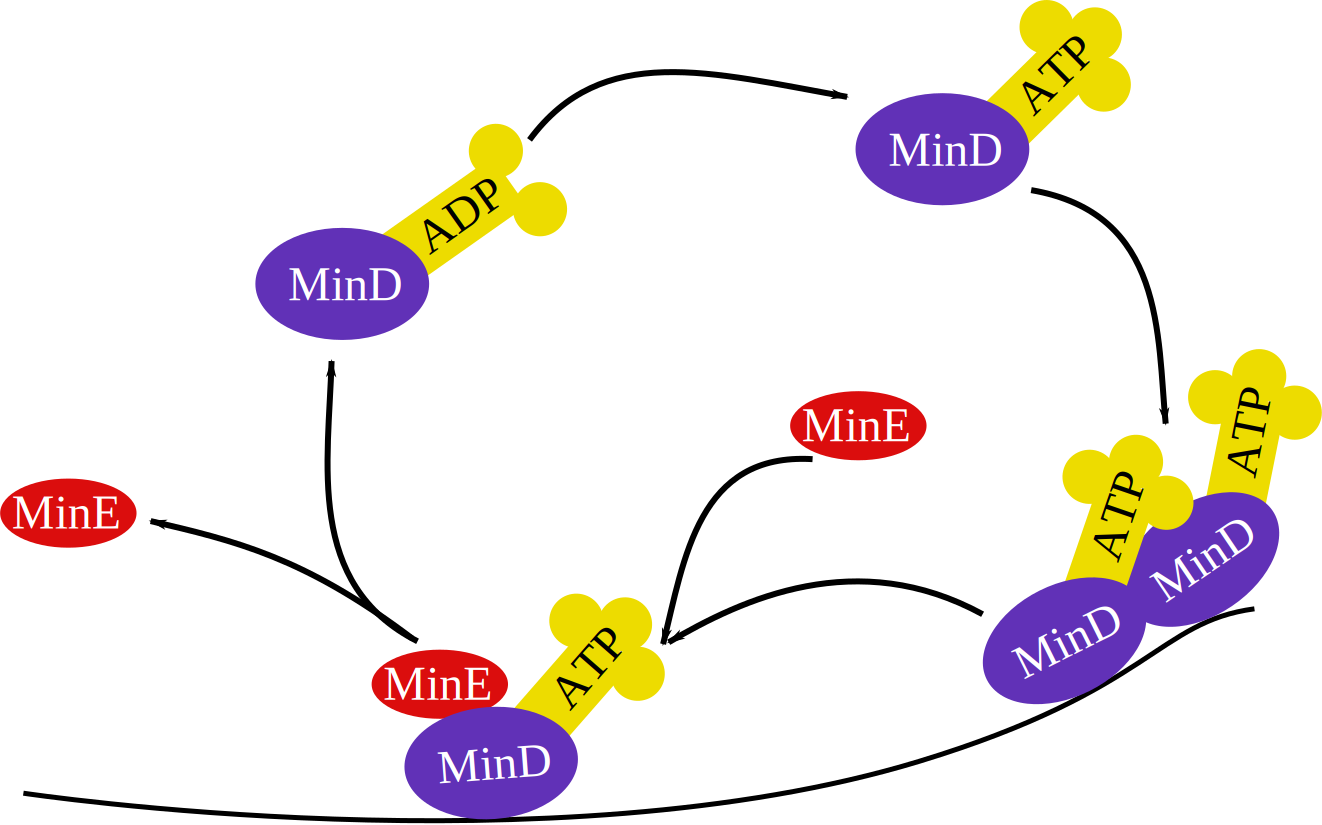
\includegraphics[width=8.7cm]{reactions}
%%   \caption{Reactions included in the model of Huang \emph{et
%%       al.}~\cite{huang2003dynamic}.}\label{fig:reactions}
%% \end{figure}

%% \begin{figure*}
%%   %\includegraphics[width=\textwidth]{../data/shape-p/3_00-0_50-0_00-0_00-15_00-exact/plots/image-plot}
%%   \begin{center}
%%     \includegraphics[width=0.8\textwidth]{../data/shape-p/3_00-0_50-0_00-0_00-15_00-exact/plots/single-image-plot}\\
%%     \vspace{-1.5em}
%%     \includegraphics[width=0.8\textwidth]{../data/shape-p/3_00-0_50-0_00-0_00-15_00-full_array/plots/single-image-plot}
%%     \vspace{-1.5em}
%%   \end{center}
%%   \caption{Images of the concentration of each protein species in a
%%     natural pill-shaped bacterium at one-second time intervals. The
%%     upper plots shows results from the deterministic model and the
%%     lower shows results from the stochastic model.  The order of
%%     frames is such that individual MinD proteins begin at the bottom
%%     of the plot (in the MinD:ATP state in the cytoplasm), and progress
%%     upward until they reach the MinE:MinD:ATP membrane-bound complex.
%%     At that point, they will spontaneously dissociate into cytoplasmic
%%     MinE (the top row) and the starting state of cytoplasmic
%%     MinD:ADP.}.
%%   \label{image-p}
%% \end{figure*}

%% \begin{figure}
%%   \includegraphics[width=8.7cm]{../data/shape-p/3_00-0_50-0_00-0_00-15_00-full_array/plots/correlation.pdf}
%%   \caption{Temporal correlation function of the total MinD found in
%%     two opposite polar regions of the pill-shaped cell, shown against
%%     the correlation time.  Data for both the the determinisitic and
%%     stochastic models are shown.  The stochastic model shows an
%%     oscillation period of 39.5 seconds and coherence time of 307 seconds.
%%     The correlation functions are scaled to have the same initial
%%     value.}
%%   \label{corr-pill}
%% \end{figure}

%% \begin{figure*}
%%   \centering
%%   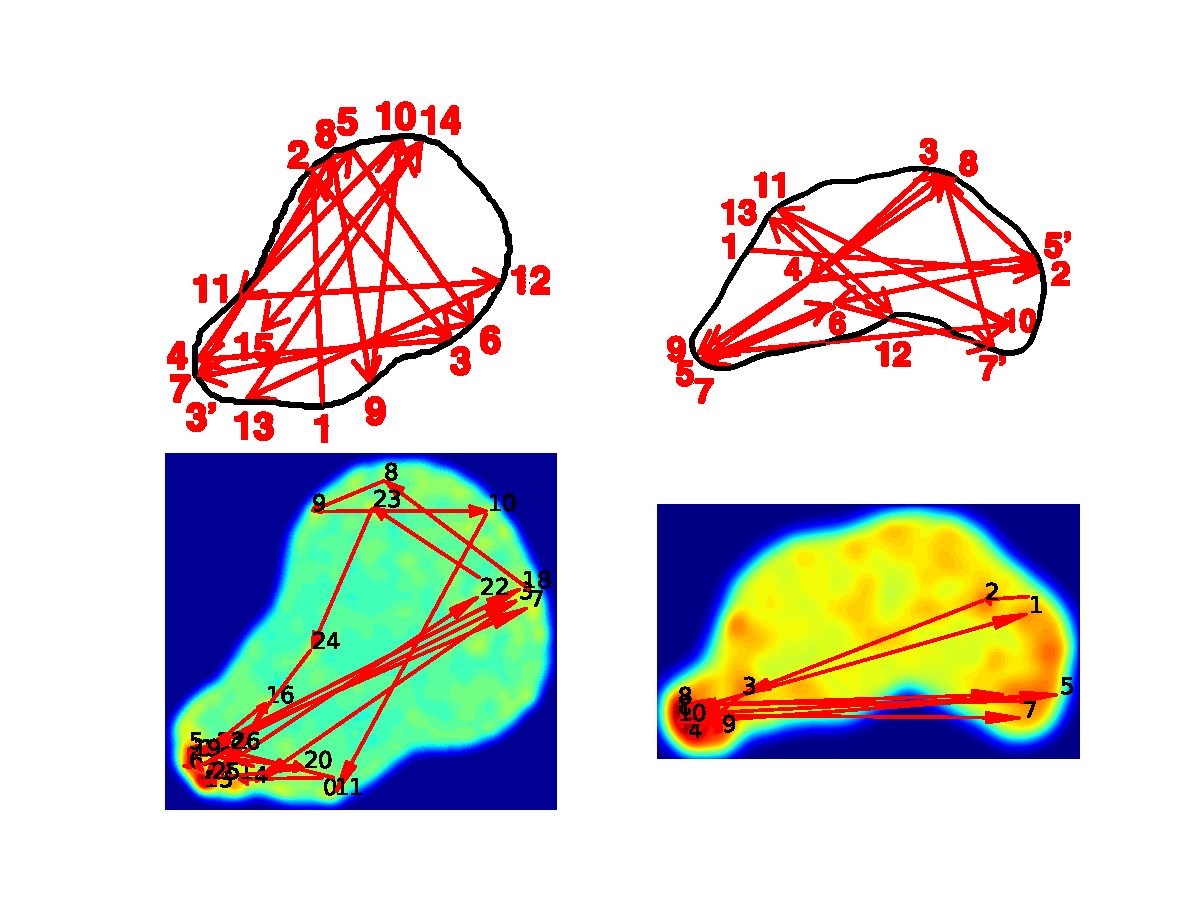
\includegraphics[width=0.8\textwidth]{../paper/plot-ave}
%%   \caption{We display here arrows depicting successive maxima in space
%%     and and time overlayed on a color plot of the total MinD density
%%     averaged over the same time period.  The simulation time covered
%%     for the flattened cells is 350 seconds, which is the same
%%     period of time depicted in the experimental data plots of Mannik
%%     \emph{et al.}~\cite{mannik2012robustness}.  For the wild-type pill
%%     shape, we only cover 250 seconds, in order to provide a
%%     useful comparison due to its shorter oscillation period.  The top
%%     row shows plots published by Mannik of the MinD maxima behavoir
%%     and the bottom two rows show our simulations using the stochastic
%%     and deterministic models, respectively.  We simulated
%%     approximations to the two shapes observed by Mannik, which we call
%%     \emph{shape A} and \emph{shape B}.  In addition, we studied two
%%     flattened stadium shapes which we call \emph{stadium A} and
%%     \emph{stadium B} corresponding in aspect ratio and thickness to
%%     the two experimental shapes.  The spatial length scale of all the
%%     figures shown was identical. Each of the flattened cell shapes
%%     uses the same color scale for the number of proteins per unit
%%     area.  Finally, we display the natural pill shape, which was also
%%     featured in Figs.~\ref{image-p} and~\ref{corr-pill}, with a
%%     different color scale to reflect the thicker cell containing more
%%     proteins per cross-sectional area.  }
%%   \label{randst-plot-ave}
%% \end{figure*}

%% \begin{figure}
%%   \includegraphics[width=8.7cm]{../data/shape-randst/0_25-18_50-18_50-95_00-15_00-full_array/plots/correlation.pdf}
%%   \includegraphics[width=8.7cm]{../data/shape-stad/0_25-2_35-1_32-0_00-15_00-full_array/plots/correlation.pdf}
%%   \caption{Temporal correlation function of the total MinD found in
%%     two opposite polar regions of the shape \emph{A} (above) and the
%%     stadium \emph{A} (below) cell shapes, shown against the
%%     correlation time.  Data for both the the determinisitic and
%%     stochastic models are shown, and the correlation functions are
%%     scaled to have the same initial value.  For shape \emph{A}, the
%%     stochastic model shows an oscillation period of 53.1 seconds and
%%     coherence time of 246 seconds, so that it takes roughly 4.6 periods
%%     for the behavoir to decohere.  For the stadium \emph{A}, the same
%%     model shows an oscillation period of 51 seconds and coherence time of
%%     323 seconds, so that it takes roughly 6.3 periods for the behavoir
%%     to decohere.}
%%   \label{fig:corr-pancake-A}
%% \end{figure}


\end{document}

